\section{Representing Multi-Modal Information}
\subsection{Learning Visual and Language Atoms}
\label{atom}
Finding the set of activity steps over large collection of videos having large visual varieties requires us to represent the semantic information in addition to the low-level visual cues. Hence, we find our language and visual atoms by using mid-level cues like object proposals and frequent words.


\paragraph{Learning Visual Atoms}
In order to learn visual atoms, we create a large collection of object proposals by independently generating object proposals from each frame of each video. These proposals are generated by using the Constrained Parametric Min-Cut (CPMC) \cite{cpmc} algorithm based on both appearance and motion cues. We note the $k^{th}$ proposal of $t^{th}$ frame of $i^{th}$ video as $r^{(i),k}_t$. Moreover, we drop the video index $(i)$ if it is clear from the context.

In order to group this object proposals into mid-level visual atoms, we follow a clustering approach. Although any graph clustering approach (\ie Keysegments \cite{keysegments}) can be applied for this problem, the joint processing of a large video collection brings additional difficulties. Images of the same objects coming from different videos have high visual differences. Hence, the basic clustering methods fail due to high inter-class variance. We propose a new method to jointly cluster object proposals from multiple videos. We defer the explanation of the clustering algorithm to Section~\ref{jointProp}.

At the end of the clustering stage, each cluster of object proposals correspond to a visual atom.

\paragraph{Learning Language Atoms}
We learn the language atoms as the salient words which occur more often than their ordinary rates based on the \emph{tf-idf} measure. We define the \emph{document} as the concatenation of all subtitles of all frames of all videos in the collection as $D=\bigcup_{i \in N_C} \bigcup_{t \in T^{(i)}} L_t^i$. Then, we follow the classical tf-idf measure and use it as $tfidf(w,D)=f_{w,D} \times \log \left( 1+ \frac{N}{n_{w}}\right)$ where $w$ is the word we are computing the tf-idf score, $f_{w,D}$ is the frequency of the word in the \emph{document} $D$, $N$ is the total number of video collections we are processing and $n_{w}$ is the number of video collections whose subtitle include the word $w$.

After computing the tf-idf, we sort all words with their tf-idf values and choose the top $K$ words as set of salient words (\emph{We set $K=100$ in our experiments}).

We show below the language atoms extracted for the activity category \emph{How to hard boil an egg?}\footnote{we include more results in the supplementary material}. The resulting collection suggests that they correspond to the important objects, actions and adjectives which represent a semantic information occurring over multiple videos.

\begin{figure}
\footnotesize
\emph{sort, place, water, egg, bottom, fresh, pot, crack, cold, cover, time, overcooking, hot, shell, stove, turn, cook, boil, break, pinch, salt, peel, lid, point, high, rules, perfectly, hard, smell, fast, soft, chill, ice, bowl, remove, aside, store, set, temperature, coagulates, yolk, drain, swirl, shake, white, roll, handle, surface, flat}
\normalsize
\caption{Language atoms learned for activity class \emph{"How to hard boil an egg?"}}
\end{figure}

\subsection{Representing Frames with Atoms}
After learning the visual and language atoms, we represent each frame via the occurrence of atoms. Formally, the representation of the $t^{th}$ frame of the $i^{th}$ video is denoted as $\mathbf{y^{(i)}_t}$ and computed as $\mathbf{y^{(i)}_t}=[\mathbf{y^{(i),l}_t},\mathbf{y^{(i),v}_t}]$ such that $k^th$ entry of the $\mathbf{y^{(i),l}_t}$ is $1$ if the subtitle of the frame has the $k^{th}$ language atom and $0$ otherwise. $\mathbf{y^{(i),v}_t}$ is also a binary vector similarly defined over visual atoms. We visualize the representation of a sample state in the Figure~\ref{visFrame}.
\begin{figure}[h!]
  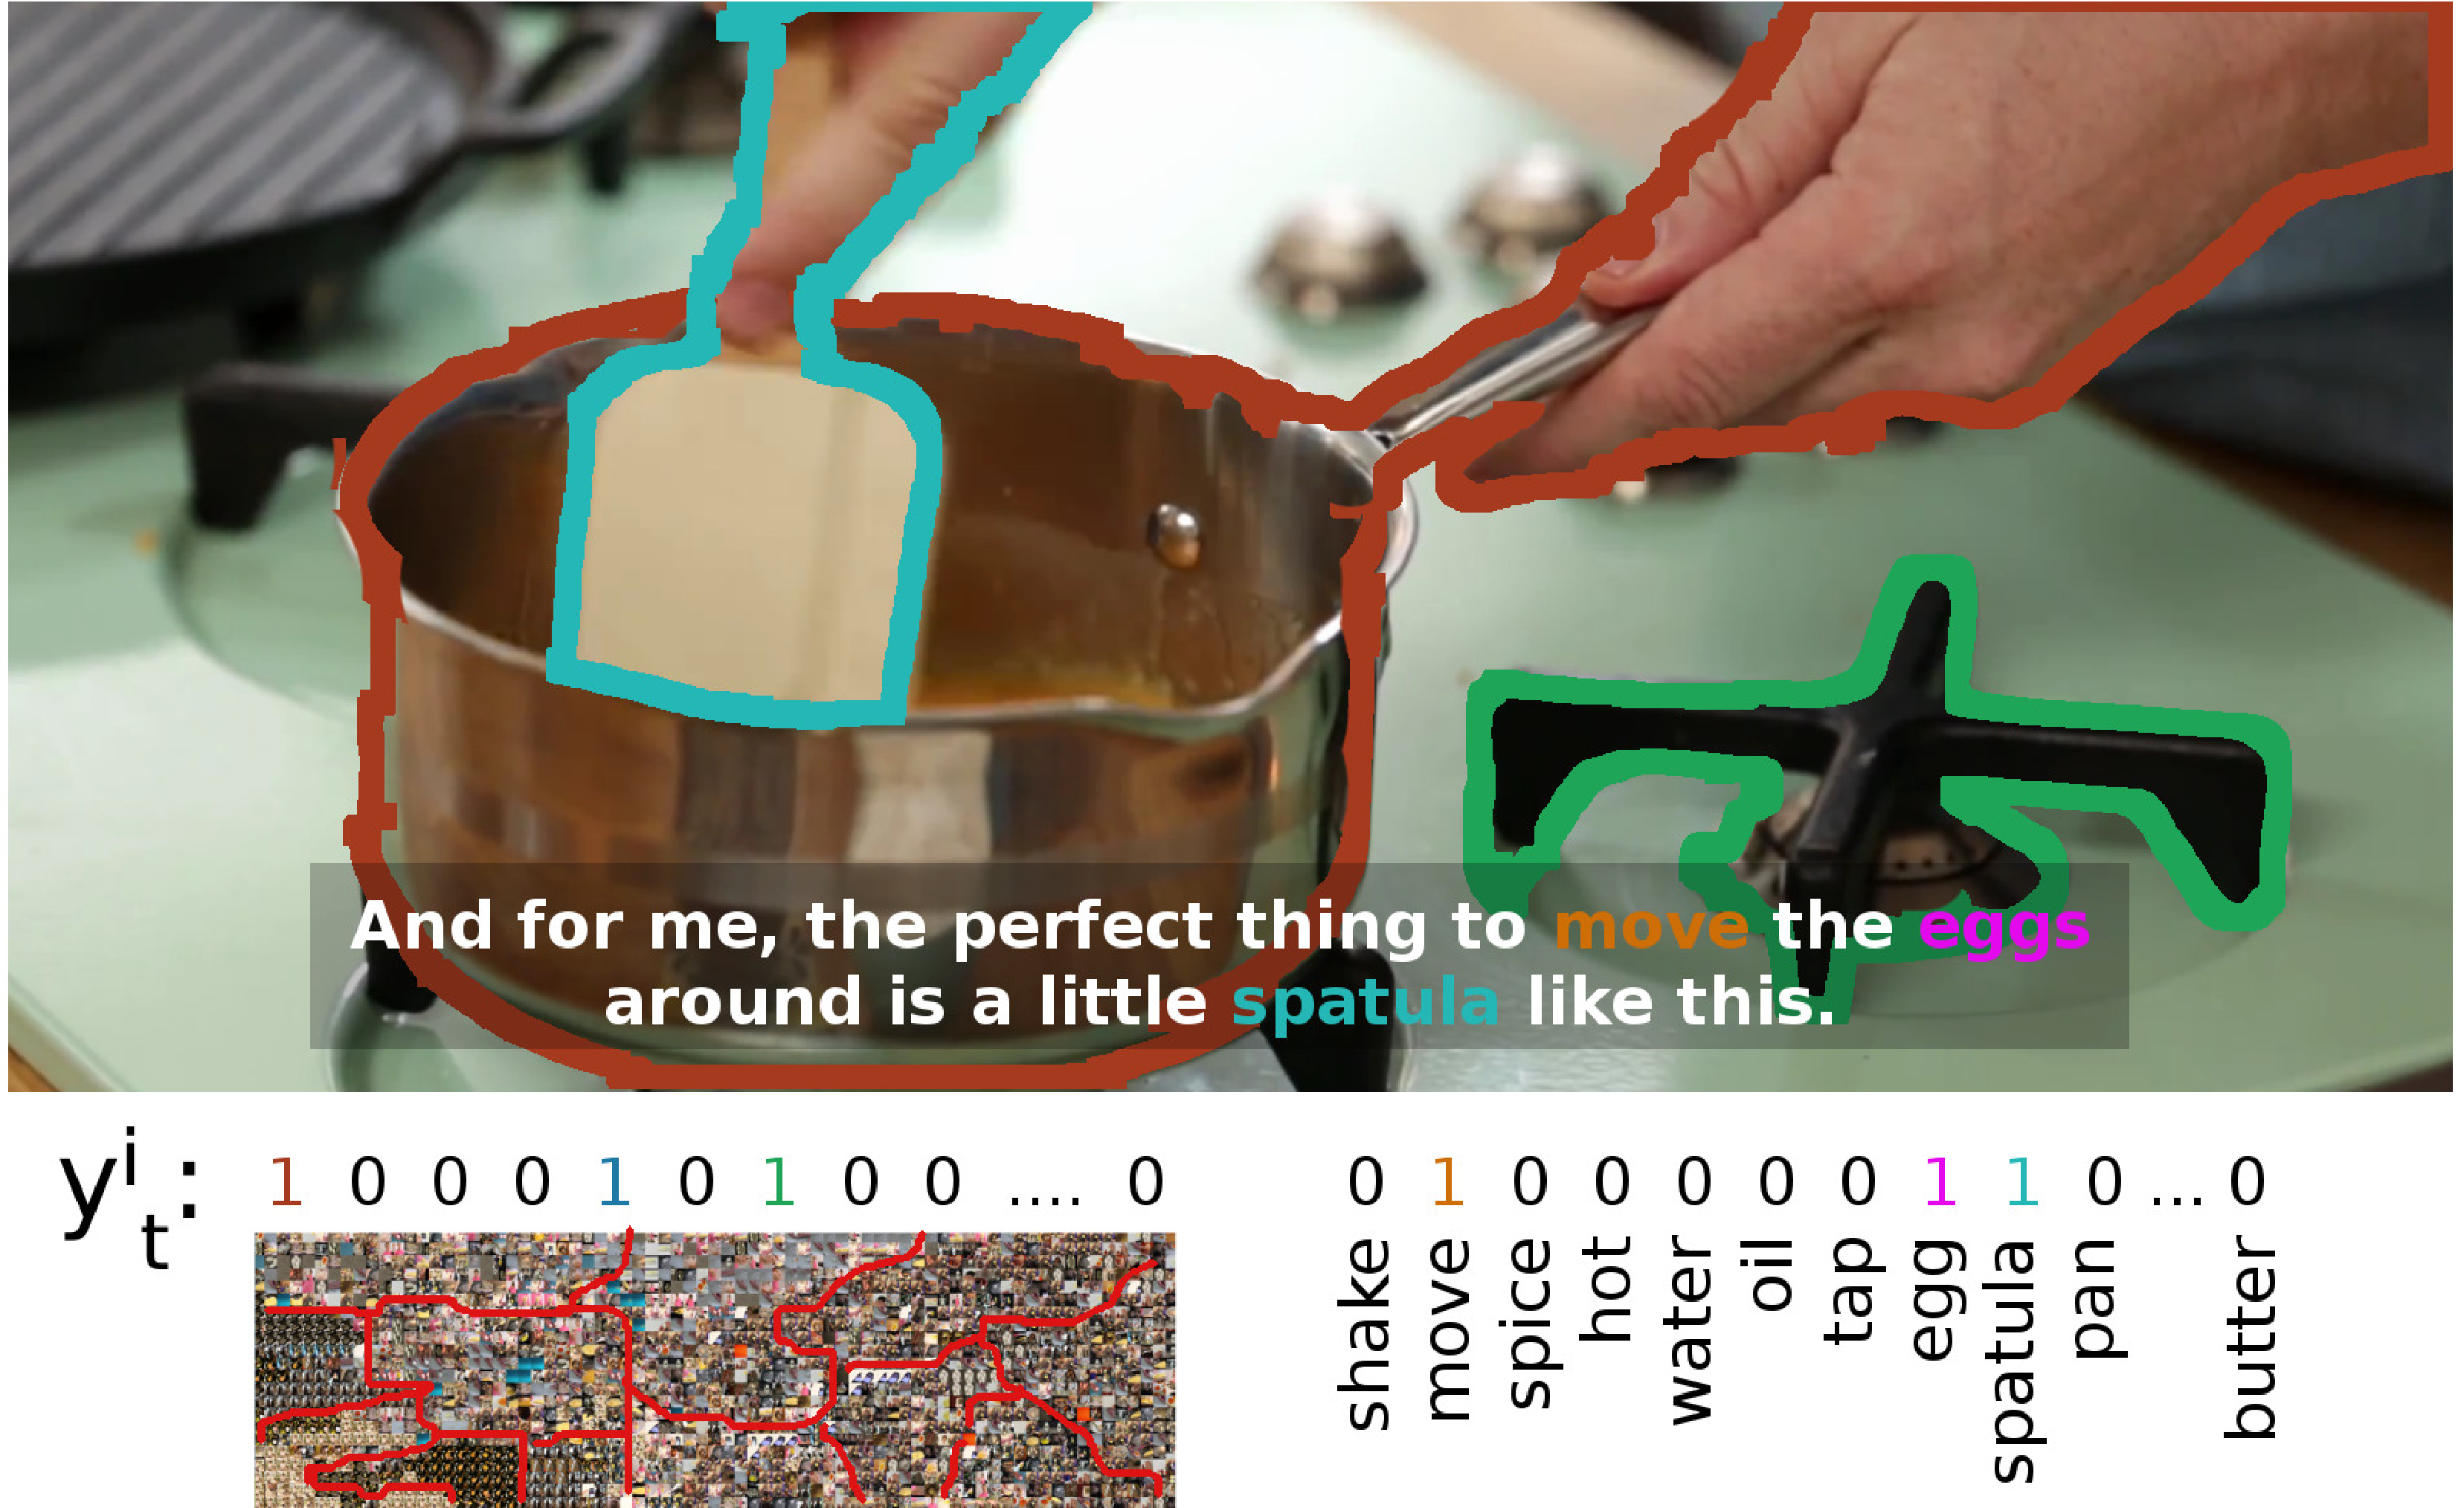
\includegraphics[width=0.48\textwidth]{frame}
  \caption{\textbf{Visualization of the representation of a sample frame.} 3 of the object proposals of the frame is included in the visual atoms and 3 of the words in the subtitle of the frame is included in the language atoms.}
  \label{visFrame}
\end{figure}

\section{Jointly Clustering Proposals From Multiple Videos}
\label{jointProp}
Given a set of object proposals generated from multiple videos, combining them into a single collection and clustering them into atoms is not desirable for two reasons; (1) semantic concepts have large visual differences among different videos and accurately clustering them into a single atom is hard, (2) atoms should contain object proposals from multiple videos in order to semantically relate videos. In order to satisfy these requirements, we propose a joint extension of the spectral clustering algorithm.

\begin{figure}[ht]
  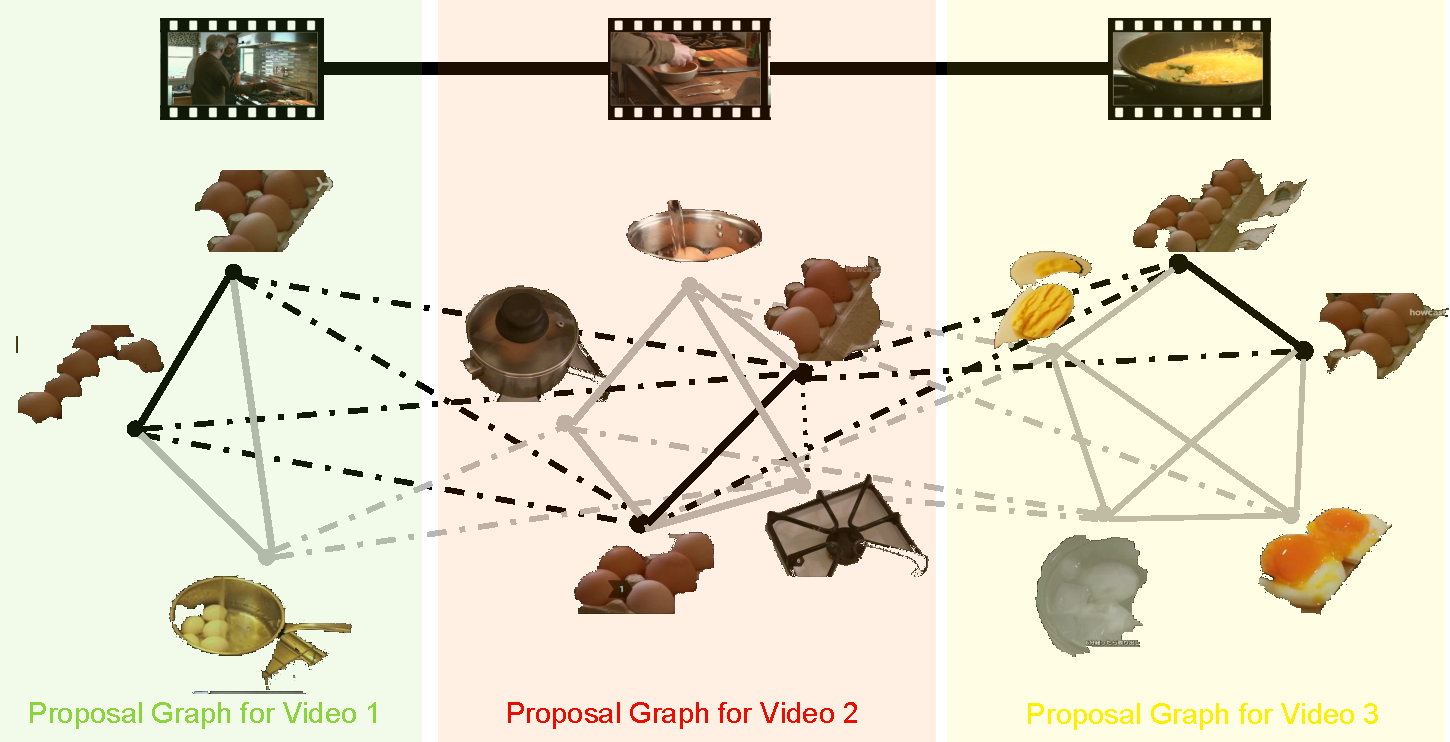
\includegraphics[width=0.48\textwidth]{joint_clustering}
  \scalebox{0.85}{

  $\arg\max  \frac{x_1^TA^{(1)}x^1}{x_1^Tx^1}+\frac{x_2^TA^{(2)}x^2}{x_2^Tx^2}+\frac{x_3^TA^{(3)}x^3}{x_3^Tx^3}+\frac{x_1^TA^{(1,2)}x^2}{x_1^T\mathds{1}\mathds{1}^Tx^2}+\frac{x_2^TA^{(2,3)}x^3}{x_2^T\mathds{1}\mathds{1}^Tx^3}$}

  %$\arg\max  \color[HTML]{BF9000}{\frac{x_1^TA^{(1)}x^1}{x_1^Tx^1}}+\color[HTML]{990000}{\frac{x_2^TA^{(2)}x^2}{x_2^Tx^2}}+\color[HTML]{38761d}{\frac{x_3^TA^{(3)}x^3}{x_3^Tx^3}}+\color[HTML]{a64d79}{\frac{x_1^TA^{(1,2)}x^2}{x_1^T\mathds{1}\mathds{1}^Tx^2}}+\color[HTML]{F1C232}{\frac{x_2^TA^{(2,3)}x^3}{x_2^T\mathds{1}\mathds{1}^Tx^3}}$}
  \caption{\textbf{Visualization of the joint proposal clustering.} Here, we show the 1NN video graph and 2NN region graph. Each region proposal is linked to its 2 nearest neighbours from the video it belongs and 2 nearest neighbours from the videos it is neighbour of. THIS NEED WORK}
  \label{hierProposal}
\end{figure}

We first explain the original spectral graph clustering algorithm and then extend it to joint clustering. Consider the set of region proposals extracted from a single video $\{r^k_t\}$, and a similarity metric $d(\cdot,\cdot)$ between any region proposal pair. We follow the single cluster graph partitioning (SCGP)\cite{scgp} approach to find the dominant cluster which maximizes the inter-cluster similarity. In other words, we solve
\begin{equation}
  \argmax_{x^k_t} \frac{\sum_{(k_1,t_1),(k_2,t_2) \in K \times T} x^{k_1}_{t_1} x^{k_2}_{t_2} d(r^{k_1}_{t_1},r^{k_2}_{t_2})}{\sum_{(k,t) \in K \times T} x^{k}_t}
\end{equation}
where, $x^{k}_t$ is a binary variable which is $1$ if $r^{k}_t$ is included in the cluster, $T$ is the number of frames and $K$ is the number of clusters per frame. When we use the vector form of the indicator variables as $\mathbf{x_{tK+k}}=x^{k}_{t}$ and the pairwise distance matrix as $\mathbf{A}_{t_1K+k_1,t_2K+k_2}=d(r^{k_1}_{t_1},r^{k_2}_{t_2})$, this equation can be compactly written as
$\argmax_{\mathbf{x}} \frac{\mathbf{x^T}A\mathbf{x}}{\mathbf{x^T}\mathbf{x}}$
Moreover, it can be solved by finding the dominant eigenvector of $\mathbf{x}$ after relaxing $x^{k}_t$ to $[0,1]$ \cite{scgp,scgp_eigen}. After finding the maximum, the remaining clusters can be found by removing the selected region proposals from the collection, and re-applying the same algorithm for the second dominant cluster.

Our extension of the SCGP into multiple videos is based on the assumption that the important objects of recipes occur in most of the videos. Hence, we re-formulate the problem by relating videos to each other. We use the kNN graph of the videos which we used for the outlier detection as explained in the Section~\ref{filter}. Moreover, we also create the kNN graph of region proposals in each video. This hierarchical graph structure is also visualized in Figure~\ref{hierProposal} for 3 videos example. After creating this graph, we choose region proposals for a cluster from each video seperately. Moreover, we impose both inter-video and intra-video similarity of chosen proposals. Main rationale behind is having seperate notion of similarity for inter-video and intra-video clusters since their visual similarity decreases drastically for intra-video case.

Given the pairwise distance matrices $\mathbf{A^{(i)}}$, binary indicator vectors $\mathbf{x^{(i)}}$ for each video and pairwise distance matrices for video pairs as $\mathbf{A^{(i,j)}}$, we define our optimization problem as;
\begin{equation}
\argmax \sum_{i \in N} \frac{\mathbf{x^{(i)^T}}\mathbf{A^{(i)}}\mathbf{x^{(i)}}}{\mathbf{x^{(i)^T}}\mathbf{x^{(i)}}} +
\sum_{i \in N} \sum_{j \in \mathcal{N}(i)} \frac{\mathbf{x^{(i)^T}}\mathbf{A^{(i,j)}}\mathbf{x^{(j)}}} {\mathbf{x^{(i)^T}}\mathds{1}\mathds{1}^T\mathbf{x^{(j)}}}
\end{equation}
where $\mathcal{N}(i)$ is the neighbours of the video $i$ in the kNN graph, $\mathds{1}$ is vector of ones and $N$ is the number of videos. We visualize this optimization objective in Figure~\ref{hierProposal} for the case of 3 videos.

Although we can not use the efficient eigen-decomposition based approach from \cite{scgp,scgp_eigen} due to the modified cost function, we can use Stochastic Gradient Descent (SGD) since the cost function is quasi-convex when it is relaxed. We use the SGD with the following analytic gradient function;
\begin{equation}
  \nabla_{\mathbf{x^{(i)}}} = \frac{2\mathbf{A^{(i)}} \mathbf{x^{(i)}} -2\mathbf{x^{(i)}} r^{(i)}}
  {\mathbf{{x^{(i)}}^T}\mathbf{x^{(i)}}}
+ \sum_{i \in N} \frac{\mathbf{A^{i,j}}\mathbf{x^{j}} - \mathbf{{x^{(j)}}^T} \mathds{1} r^{(i,j)}}{\mathbf{{x^{(i)}}^T} \mathds{1} \mathds{1}^T \mathbf{x^{(j)}} }
  %\text{Some vector matrix multiplication}
\end{equation}

where $r^{(i)}=\frac{\mathbf{x^{(i)^T}}\mathbf{A^{(i)}}\mathbf{x^{(i)}}}{\mathbf{x^{(i)^T}}\mathbf{x^{(i)}}}$ and $r^{(i,j)}=\frac{\mathbf{x^{(i)^T}}\mathbf{A^{(i,j)}}\mathbf{x^{(j)}}} {\mathbf{x^{(i)^T}}\mathds{1}\mathds{1}^T\mathbf{x^{(j)}}}$

After finding the dominant cluster by optimizing the cost function, we remove the selected cluster and re-apply the same algorithm to find the next dominant cluster. After finding $K=20$ clusters, we discard the remaining region proposals. In Figure~\ref{cvis}, we visualize some of the clusters which our algorithm generated after applied on the videos returned by the query \emph{How to Hard Boil an Egg}. As shown the figure, the resulting clusters are highly correlated and correspond to semantic objects\&concepts.
\begin{figure}[ht]
  \begin{subfigure}[b]{0.23\textwidth}
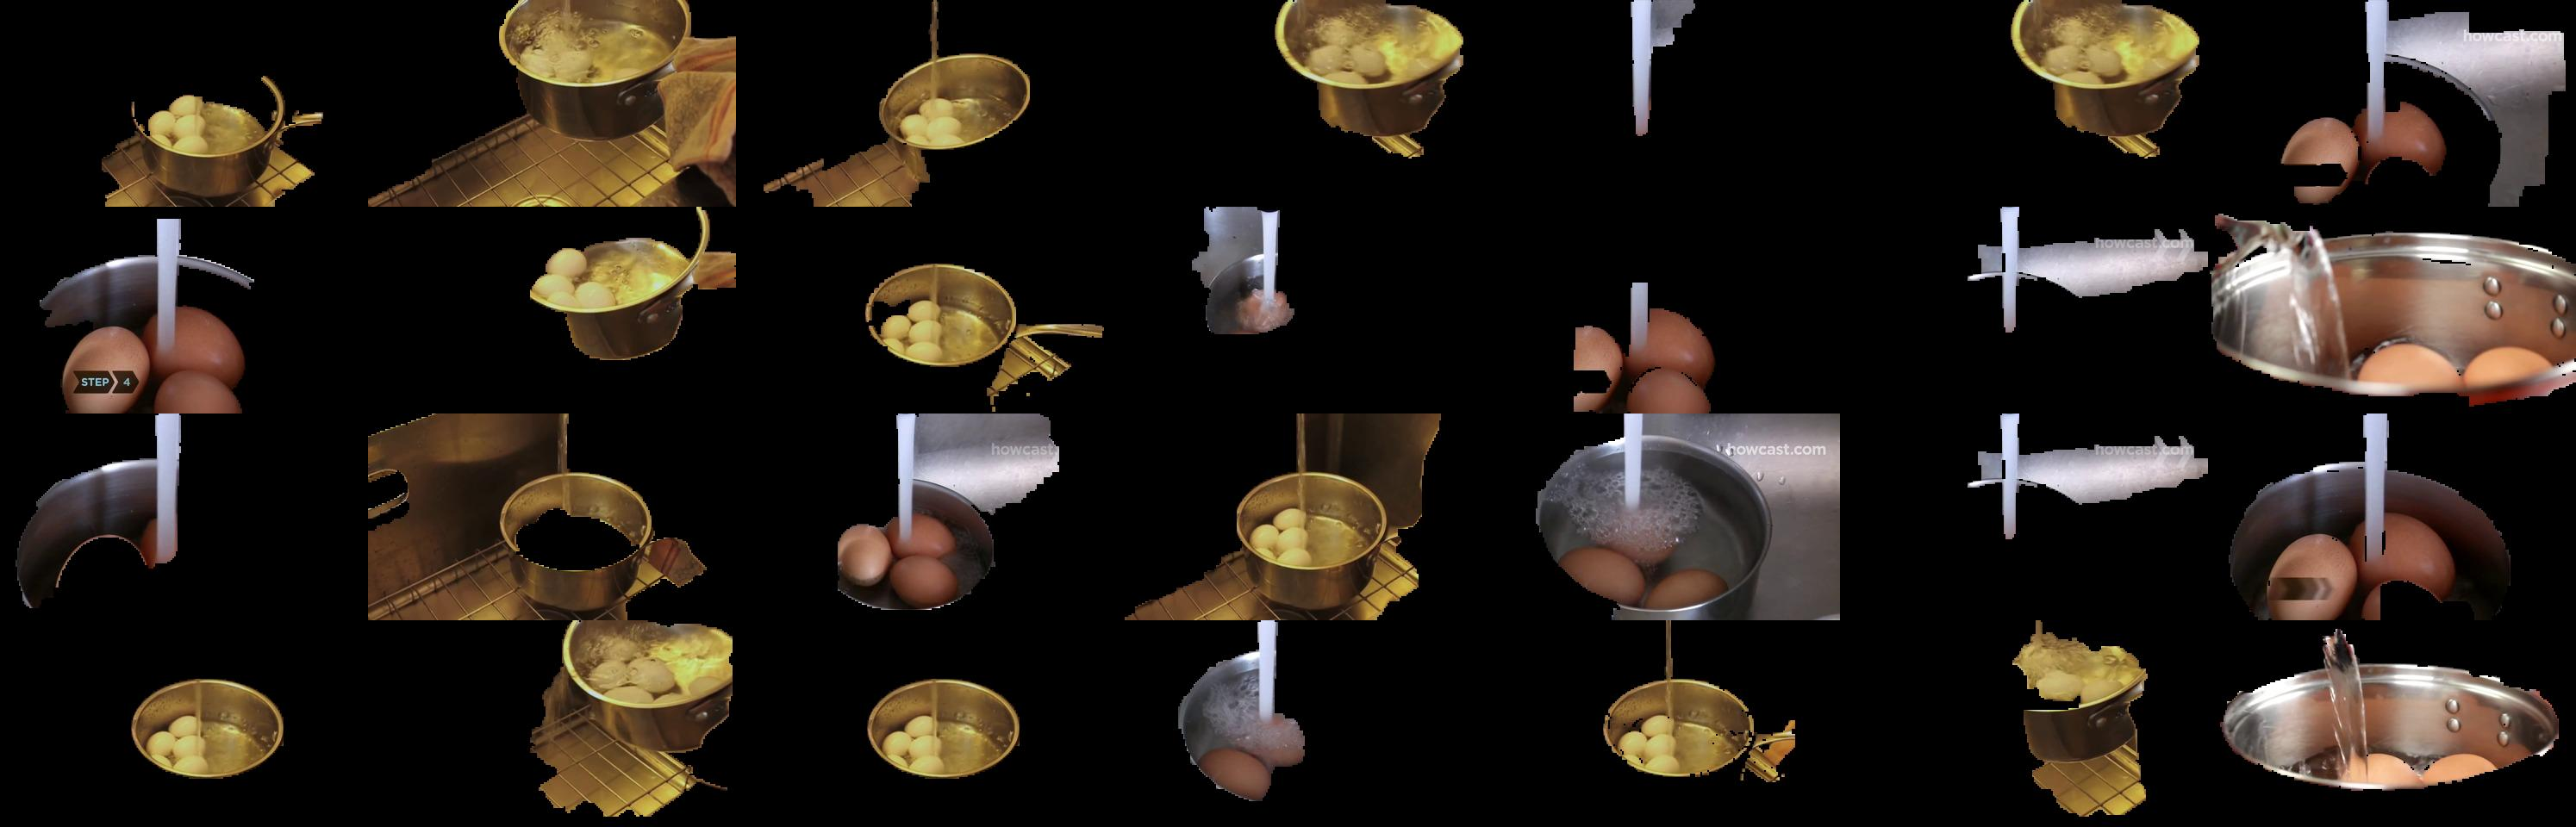
\includegraphics[width=\textwidth]{im0.png}
%\caption{Cluster 1}
\end{subfigure}
~
\begin{subfigure}[b]{0.23\textwidth}
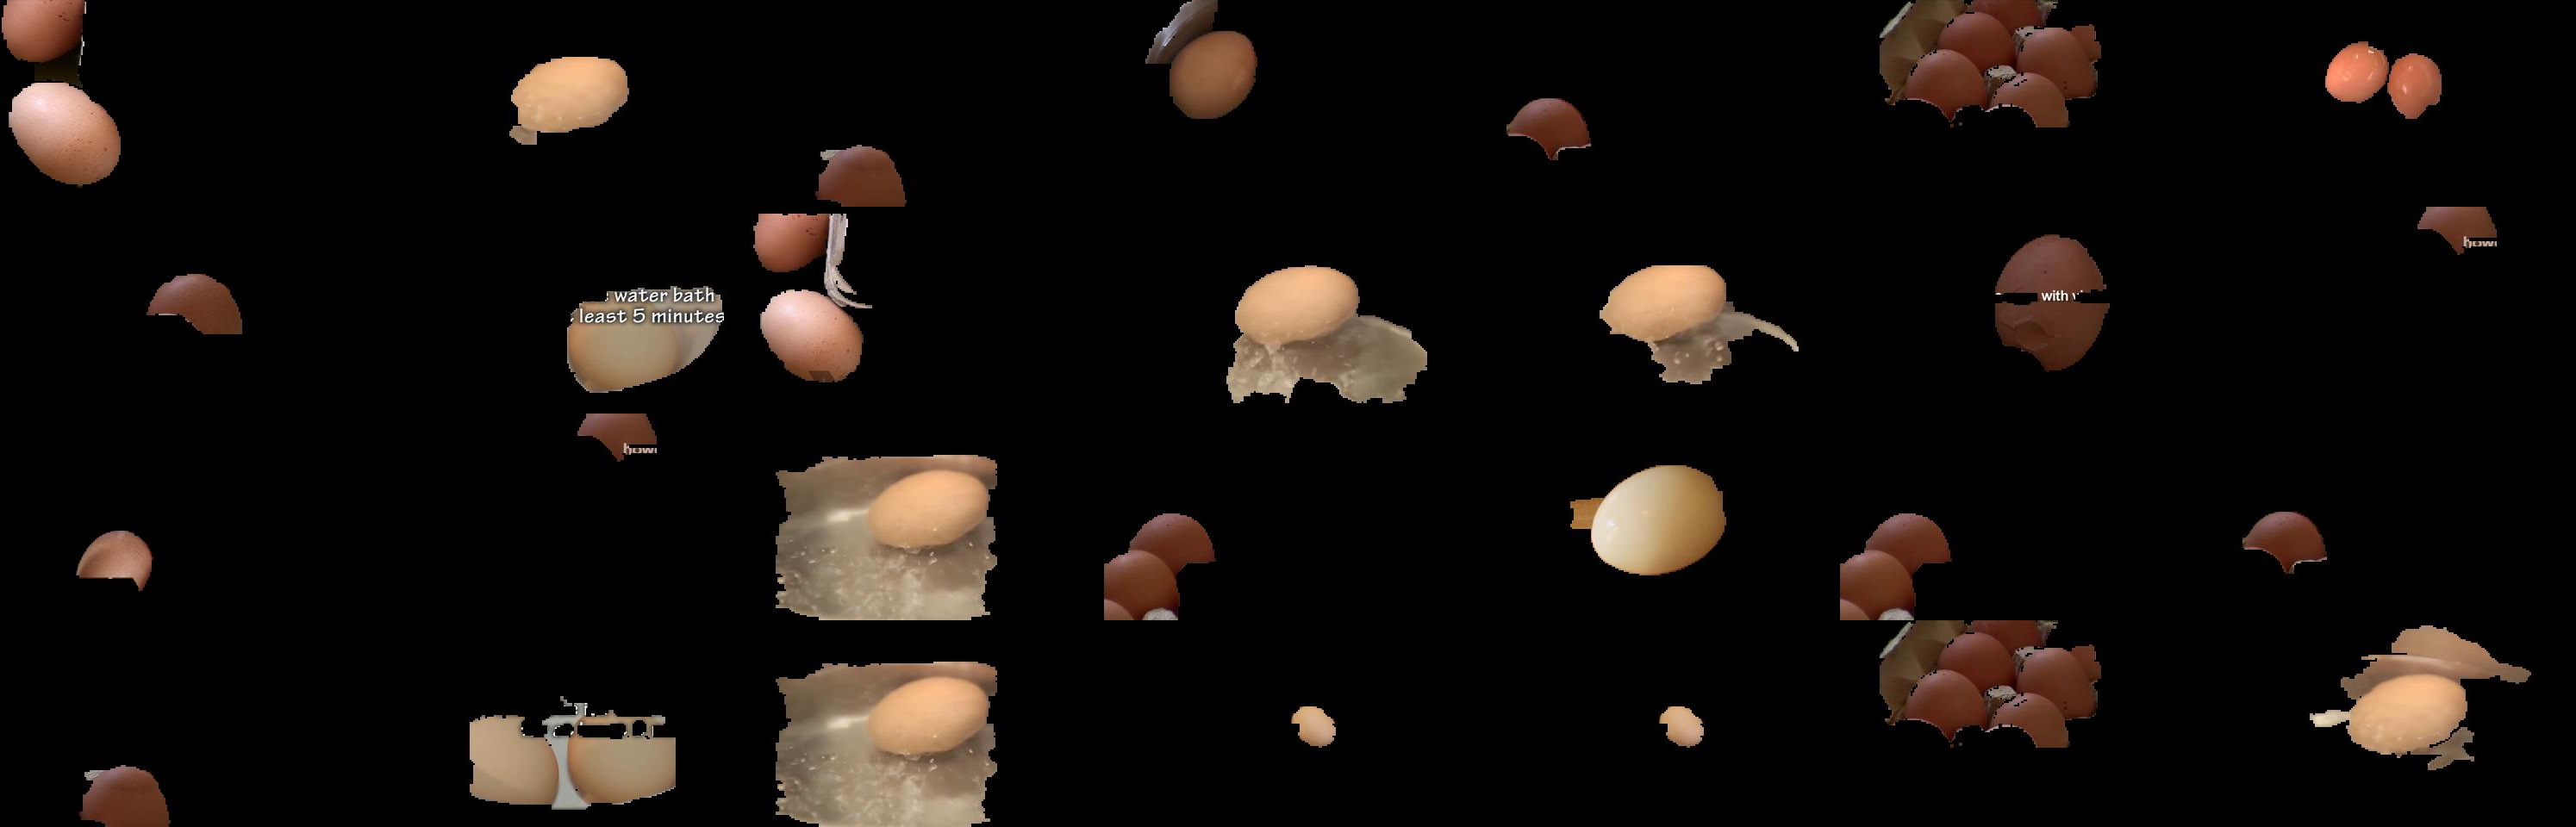
\includegraphics[width=\textwidth]{im4.png}
%\caption{Cluster 2}
\end{subfigure}
\begin{subfigure}[b]{0.23\textwidth}
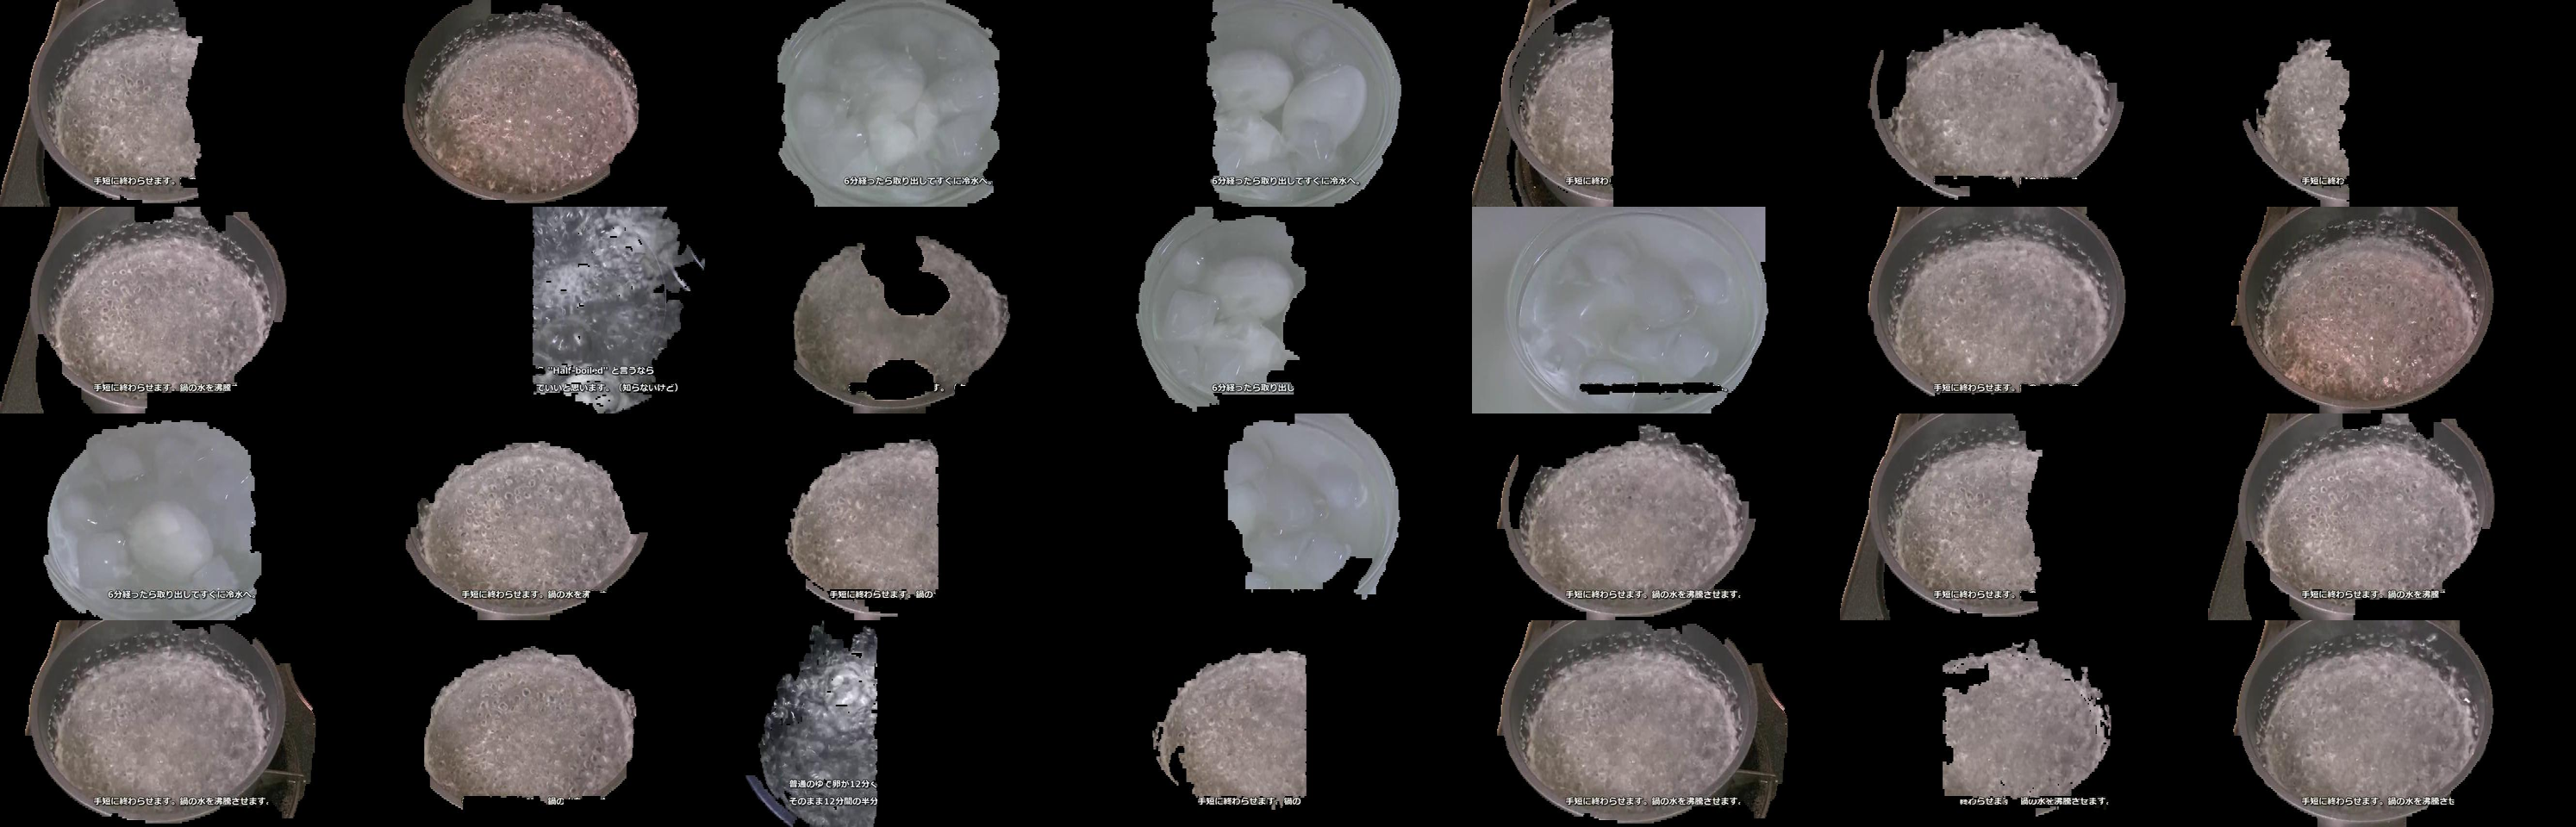
\includegraphics[width=\textwidth]{im5.png}
\end{subfigure}
~
\begin{subfigure}[b]{0.23\textwidth}
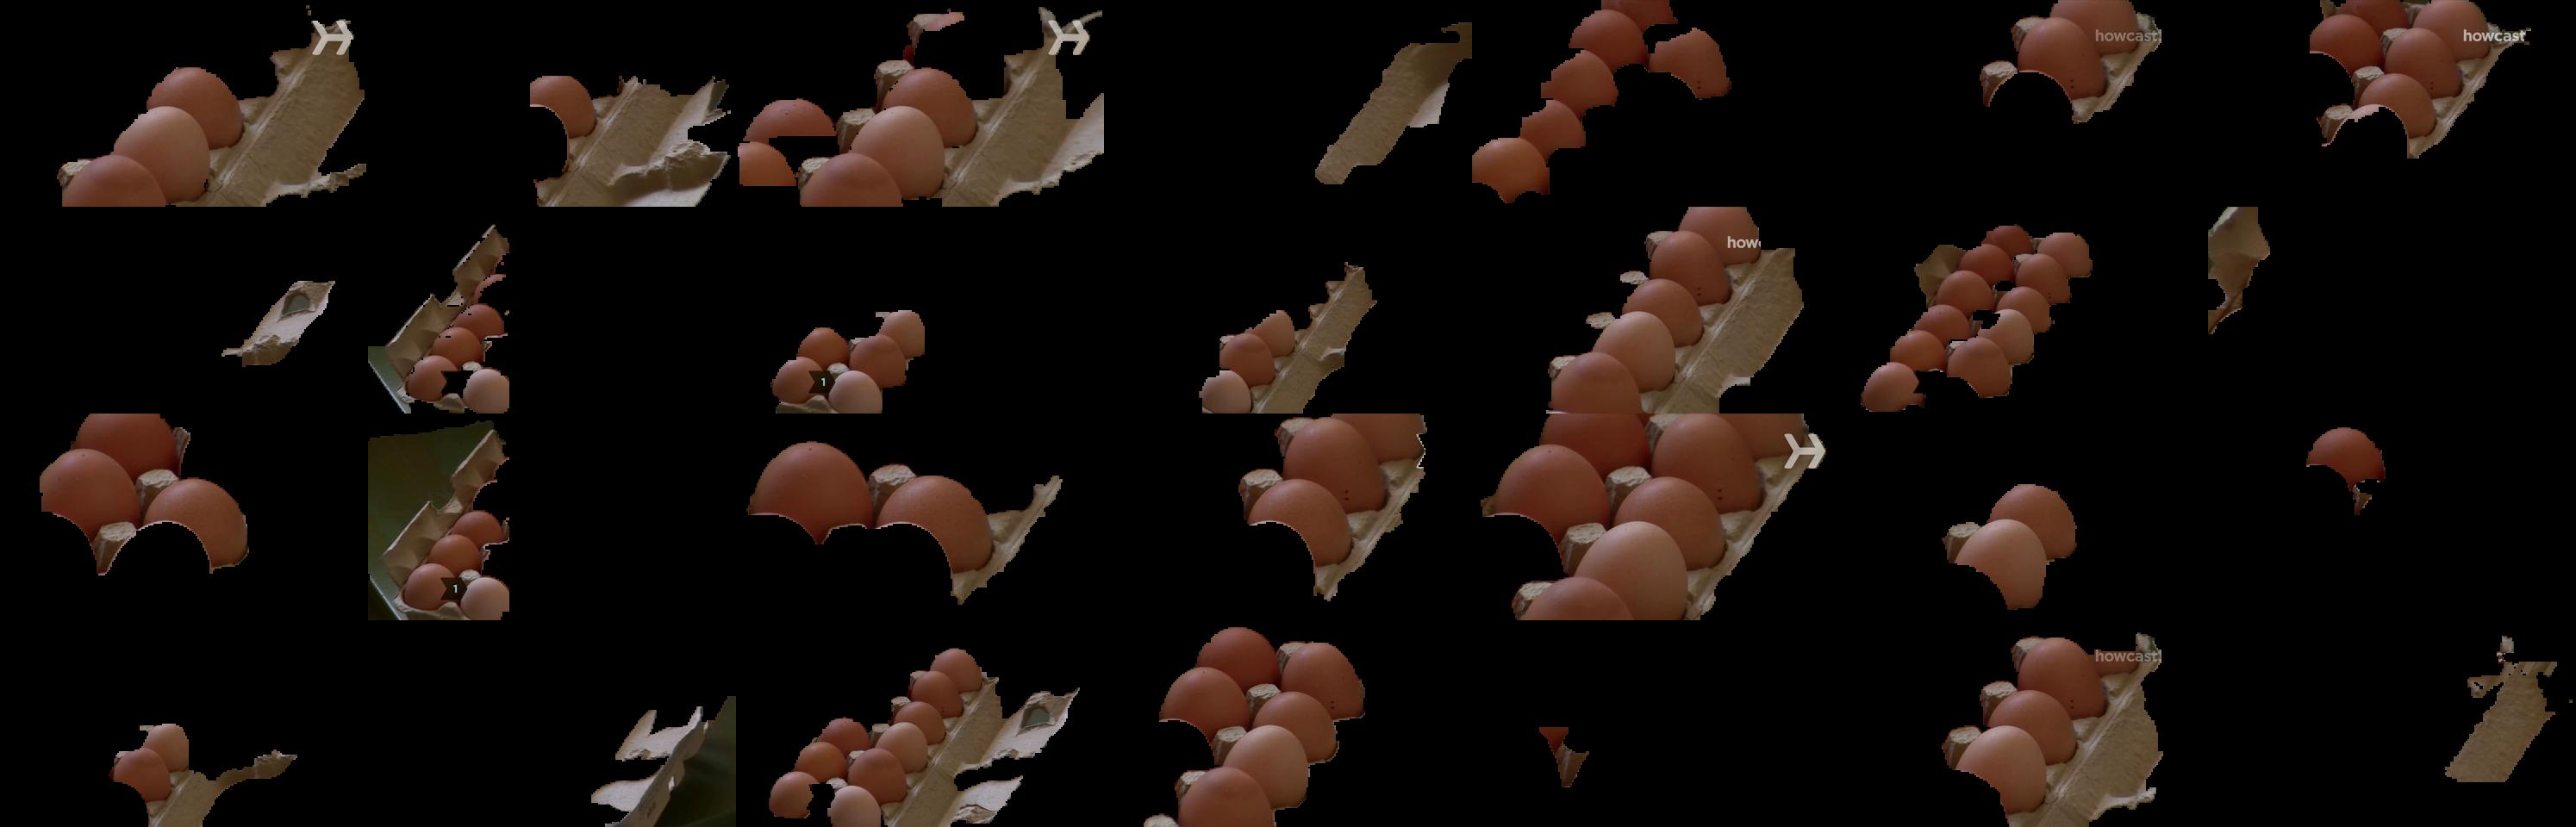
\includegraphics[width=\textwidth]{im7.png}
\end{subfigure}

\begin{subfigure}[b]{0.23\textwidth}
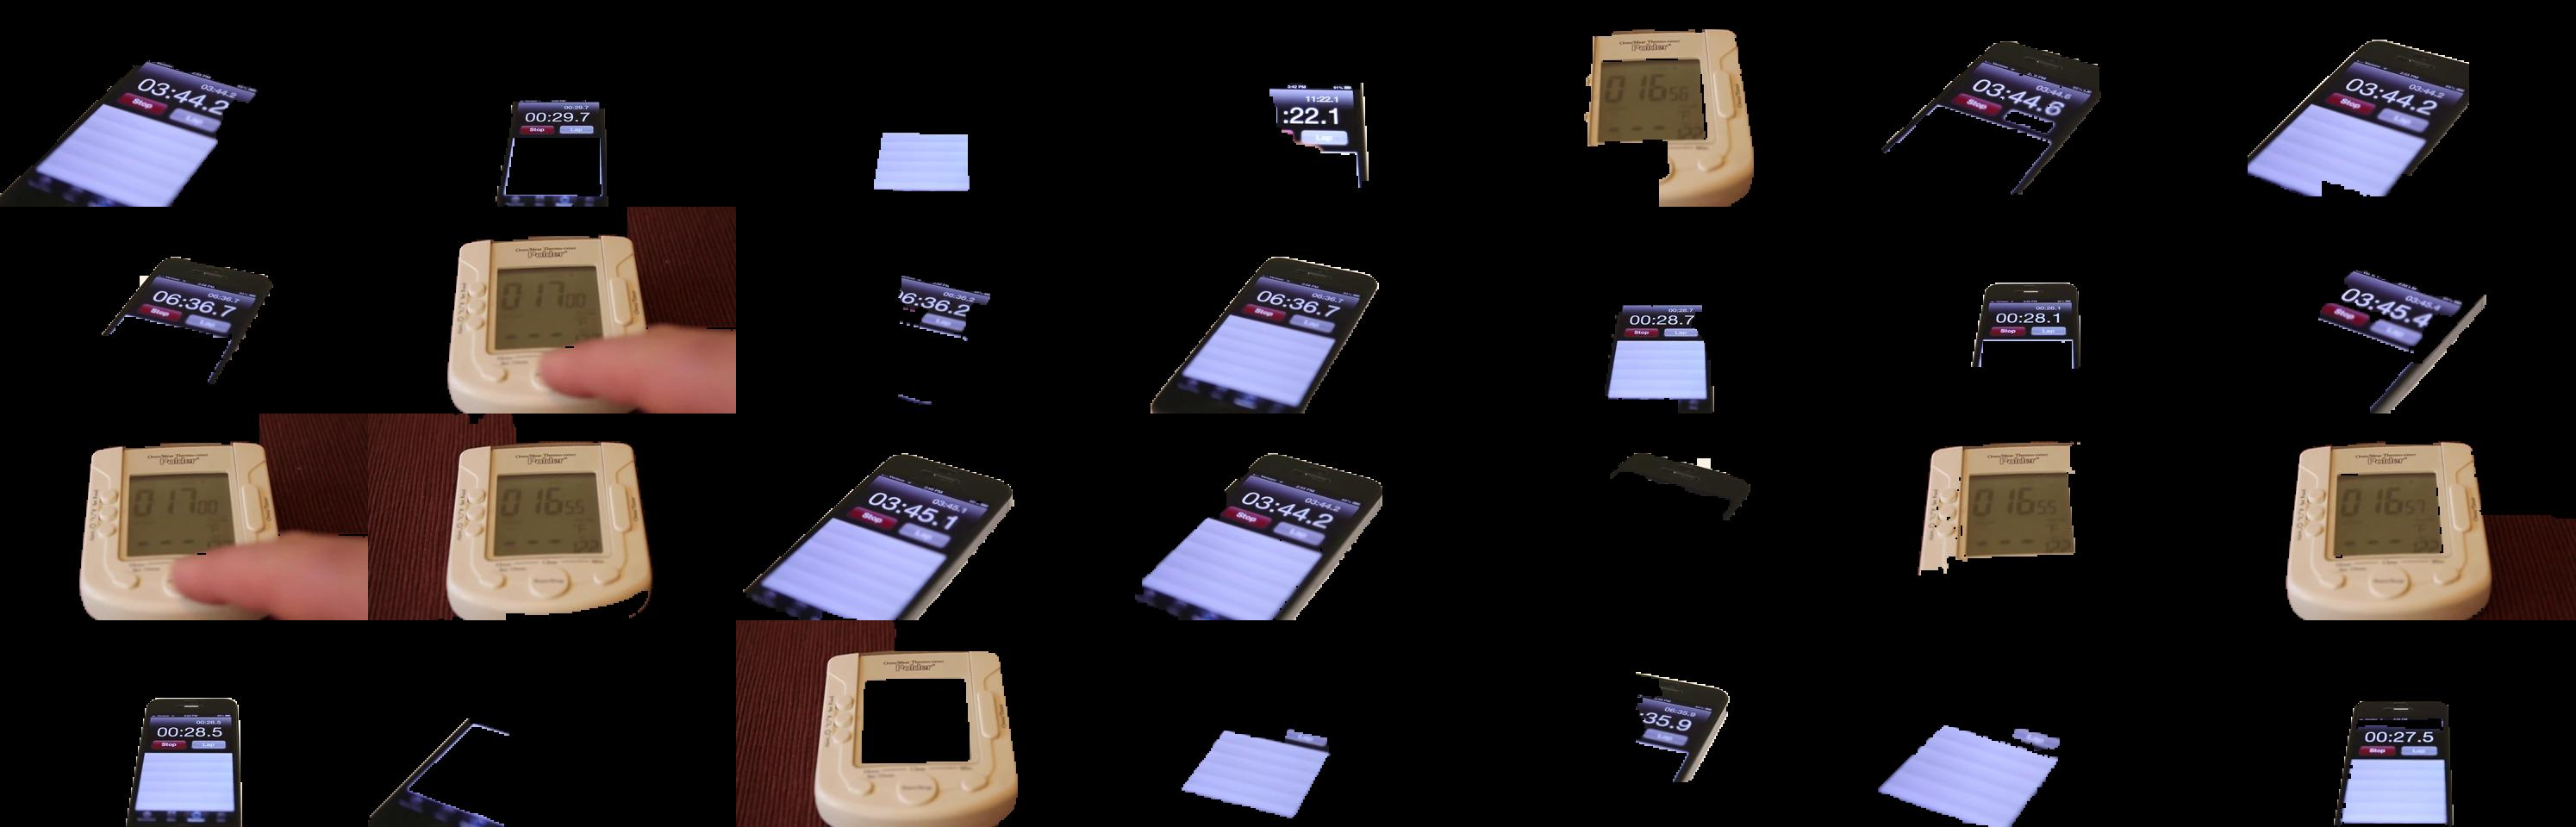
\includegraphics[width=\textwidth]{im8.png}
\end{subfigure}
~
\begin{subfigure}[b]{0.23\textwidth}
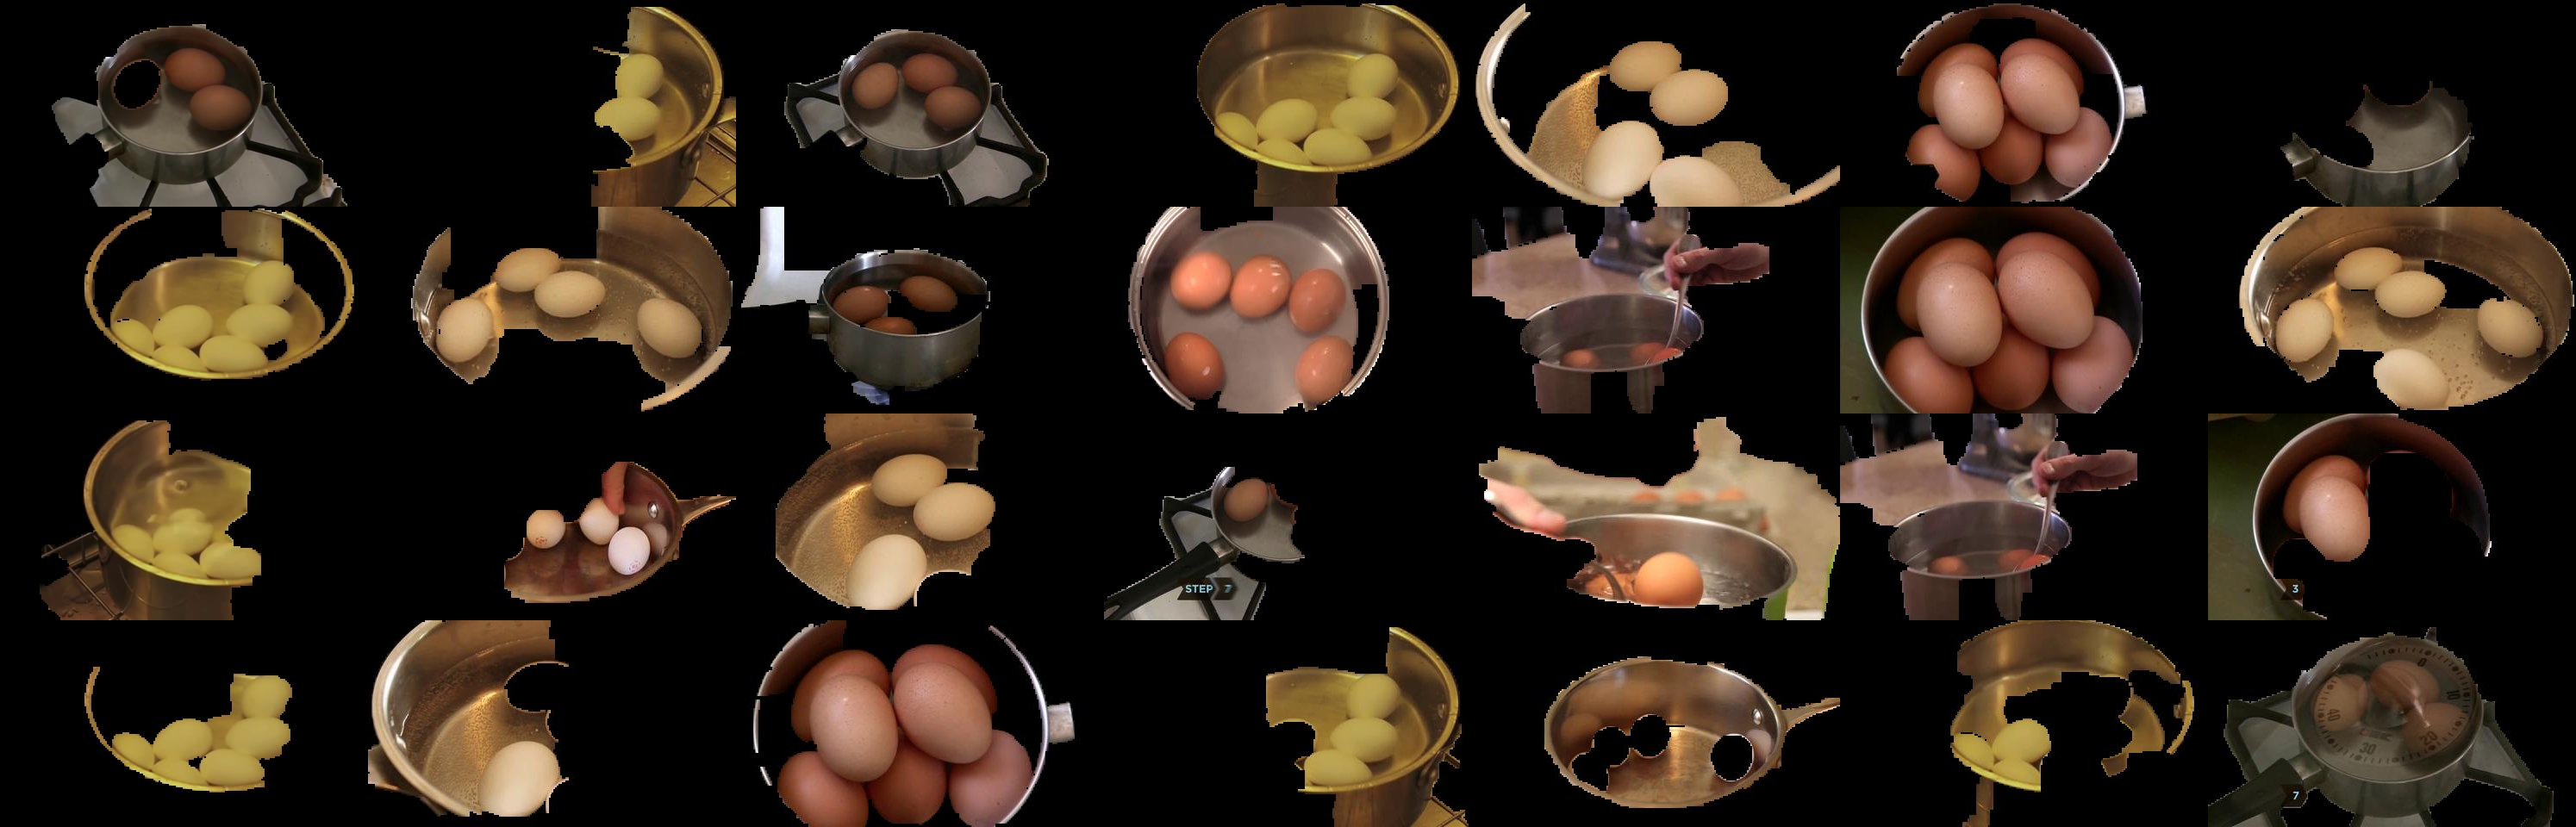
\includegraphics[width=\textwidth]{im10.png}
\end{subfigure}
\caption{Randomly selected images of randomly selected clusters learned for \emph{How to hard boil an egg?}}
\label{cvis}
\end{figure}
